\documentclass[aspectratio=43]{beamer}

\usepackage{dtucolors}
\usepackage[T1]{fontenc}
\usepackage[utf8]{inputenc}
\usepackage[english]{babel}
\usepackage{pgfplots}
\pgfplotsset{compat=newest}
\usepackage{booktabs}
\usepackage{siunitx}
\usepackage{listings}

% Listings
\lstset{
    basicstyle=\scriptsize\ttfamily,% the size of the fonts that are used for the code
    breakatwhitespace=false,          % sets if automatic breaks should only happen at whitespace
    breaklines=true,                  % sets automatic line breaking
    captionpos=b,                     % sets the caption-position to bottom
    commentstyle=\color{s14a},        % comment style
    deletekeywords={},                % if you want to delete keywords from the given language
    escapeinside={\%*}{*)},           % if you want to add LaTeX within your code
    frame=single,                     % adds a frame around the code
    keywordstyle=\bfseries\ttfamily\color{s09}, % keyword style
    language=Python,                  % the language of the code
    morekeywords={*,...},             % if you want to add more keywords to the set
    numbers=left,                     % where to put the line-numbers; possible values are (none, left, right)
    numbersep=5pt,                    % how far the line-numbers are from the code
    numberstyle=\sffamily\tiny\color{dtugray}, % the style that is used for the line-numbers
    rulecolor=\color{dtugray},        % if not set, the frame-color may be changed on line-breaks within not-black text (e.g. comments (green here))
    showspaces=false,                 % show spaces everywhere adding particular underscores; it overrides 'showstringspaces'
    showstringspaces=false,           % underline spaces within strings only
    showtabs=false,                   % show tabs within strings adding particular underscores
    stepnumber=1,                     % the step between two line-numbers. If it's 1, each line will be numbered
    stringstyle=\color{s07},          % string literal style
    tabsize=2,                        % sets default tabsize to 2 spaces
    title=\lstname,                   % show the filename of files included with \lstinputlisting; also try caption instead of title
}

\lstdefinestyle{usecase}{
  emptylines=1,
  breaklines=true,
  basicstyle=\ttfamily\color{black},
  escapeinside={@}{@},
  keywordstyle=\bfseries,
  morekeywords = {Scenario, Postconditions, Preconditions}
}

\lstdefinestyle{Dart}{
  language=Java, 
  emptylines=1,
  breaklines=true,
  escapeinside={@}{@},
  morekeywords = {async}
}

\definecolor{mygreen}{rgb}{0,0.6,0}
\definecolor{mygray}{rgb}{0.4,0.4,0.4}
\definecolor{mymauve}{rgb}{0.58,0,0.82}

% Define colors used for listings
\definecolor{dkgreen}{rgb}{0,0.6,0}
\definecolor{dkred}{rgb}{0.6,0,0}
\definecolor{gray}{rgb}{0.5,0.5,0.5}
\definecolor{mauve}{rgb}{0.58,0,0.82}

%Reuse images from thesis.
\newcommand{\imgdir}{../Thesis/img/}

% Latin Modern
\usepackage{lmodern}
% Verdana font type
%\usepackage{verdana}
% Helvetica
%\usepackage{helvet}
% Times (text and math)
%\usepackage{newtx, newtxmath}

\usetheme[department=compute]{DTU}

\title[Requirements as tests]{Requirements as tests}
\author{Kim Rostgaard Christensen}
\institute{Technical University of Denmark (DTU)}
\date{\today}
	
\newcommand{\tabitem}{{\color{dtured}$\bullet$} }

\begin{document}
\frame{
	\maketitle
}

\frame{
	\frametitle{Outline}
	\tableofcontents
}

\section{Problem domain}
\subsection{Problem statement}
\frame{
	\frametitle{Problem statement}
	
	\begin{block}{High failure rate in software projects}
%TODO Find reference to why software projects fail.
	  Causes points to requirements being:
		\begin{itemize}
			\item Incomplete
            \item Under-specified
			\item Unaligned
		\end{itemize}
	\end{block}
	
}

\subsection{Figure/stuff}
\frame{
	\frametitle{Flow}
\begin{figure}[!htbp]
\centering
\includegraphics[width=0.7\textwidth]{\imgdir ideal_flow}
\caption{Ideal development flow}
\label{fig:ideal_flow}
\end{figure}
}


\begin{figure}[!htbp]
\centering
\includegraphics[width=0.5\textwidth]{\imgdir tests-relation-to-implementation}
\caption{Concept of mapping from requirements to implementation}
\label{fig:tests-relation-to-implementation}
\end{figure}

\begin{figure}[!htbp]
\centering
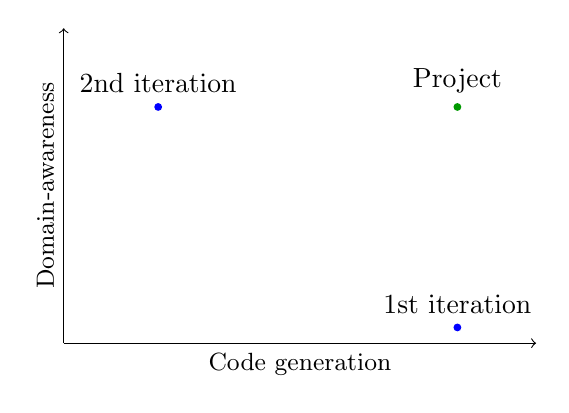
\begin{tikzpicture}

% horizontal axis
\draw[->] (0,0) -- (6,0) node[anchor=north,midway] {\small Code generation};

% vertical axis
\draw[->] (0,0) -- (0,4) node[anchor=south,rotate=90,midway] {\small Domain-awareness};

\draw (5,0.2) node[circle,fill,inner sep=1pt, fill=blue, label=above:1st iteration] {};
\draw (1.2,3.0) node[circle,fill,inner sep=1pt, fill=blue, label=above:2nd iteration] {};

% Project dot
\draw (5,3) node[circle,fill,inner sep=1pt, fill=dkgreen, label=above:Project] {}; 

\end{tikzpicture}
\caption{Project parameters and key points}
\label{fig:project_parameter_plot}
\end{figure}


\begin{figure}[!htbp]
  \centering
  \includegraphics[scale=0.6]{\imgdir sor-model}
  \caption{Stimuli-organism-response model. Used -- for instance -- in psychology, but is analogous to black-box testing}
  \label{fig:sor-model}
\end{figure}


\begin{figure}[!htbp]
\centering
\includegraphics[scale=0.6]{\imgdir test-driven-development-flow}
\caption{Basic work-flow of test-driven development}
\label{fig:test-driven-development-flow}
\end{figure}

\begin{figure}[ht]
\centering
\includegraphics[width=0.9\textwidth]{\imgdir component_diagram}
\caption{Component diagram}
\label{fig:component_diagram}
\end{figure}

\begin{figure}[ht]
\centering
\includegraphics[width=0.6\textwidth]{\imgdir receptionist_workflow}
\caption{Labeled activity diagram of the basic workflow of a receptionist}
\label{fig:receptionist-workflow}
\end{figure}

%The concepts

\begin{figure}[!htbp]
  \centering
  \includegraphics[width=0.70\textwidth]{\imgdir markdown_ui_mockup}
  \caption{Crude mock-up of a user interface using a markup language for writing use cases}
\label{fig:markdown_ui_mockup}
\end{figure}

\begin{figure}[!htbp]
\includegraphics[scale=0.4]{\imgdir test_case_ui}
\centering
\caption{Use case editor UI mockup}
\label{fig:use_case_editor_mockup}
\end{figure}

\includegraphics[width=0.4\textwidth]{\imgdir customer-ui-mockup-use-cases}

%Meta models
\begin{figure}[h]
  \centering
  \includegraphics[scale=0.72]{\imgdir concept2_use_case_meta_model}
  \caption{Partial meta model for creating use cases models in concept 2}
  \label{fig:concept2_use_case_meta_model}
\end{figure}

\begin{figure}[!htbp]
  \centering
  \includegraphics[scale=0.72]{\imgdir concept2_use_case_mapping}
  \caption{Concept 2 use case mapping}
  \label{fig:concept2_use_case_mapping}
\end{figure}


\begin{figure}[!htbp]
  \centering
  \includegraphics[scale=0.9]{\imgdir 3rd_iteration_meta_model}
  \caption{Meta model of the third concept}
  \label{fig:3rd_iteration_meta_model}
\end{figure}

\begin{lstlisting}[style=Dart, caption=Test code for single call allocation,label={lst:test-code-single-call-allocation}]
  static void pickupAllocatedCall(Receptionist receptionist, 
                                  Receptionist receptionist2, 
                                  Customer callee) {
    String receptionNumber = '12340002';
    Model.Call allocatedCall;
    
    log.info ('Customer ${callee.name} dials ${receptionNumber}');
    callee.dial (receptionNumber);
    log.info ('Receptionist ${receptionist.user.name} hunts call.');
    allocatedCall = receptionist.huntNextCall();
   
    expect (receptionist2.pickup(call), throwsA(Forbidden));
    log.info('Test done');
  }
\end{lstlisting}


\end{document}